% fithesis2 with modifications used, please use local fithesis.cls file, not system-wide installed.
\documentclass[11pt,oneside,final]{fithesis2}
% \documentclass[oneside,final]{fithesis2}
% \usepackage[resetfonts]{cmap}
\usepackage{lmodern}

\usepackage[english]{babel}
\usepackage[utf8x]{inputenc}
%\usepackage[IL2]{fontenc}
\usepackage[T1]{fontenc}

\usepackage{hyperref}
\usepackage{graphicx}
\usepackage{color}
\usepackage{afterpage}
\usepackage{calc}
\usepackage{subfig}
\usepackage{amssymb}
\usepackage{amsthm}
\usepackage{amsmath}
%\usepackage{titlesec}

% floating for figures H
\usepackage{float}
\restylefloat{figure}

% \usepackage{sistyle}

% some symbols in package
% \usepackage{textcomp}
% \usepackage{inputenx}

% text super/sub scripts
\usepackage{fixltx2e}

% % algpseudocode was not installed by default; http://ctan.org/pkg/algorithmicx
% % http://tex.stackexchange.com/questions/38978/how-can-i-manually-install-a-latex-package-debian-ubuntu-linux
% % http://ftp.cstug.cz/pub/tex/CTAN/macros/latex/contrib/algorithmicx/algorithmicx.pdf
\usepackage{algpseudocode}

% \usepackage[options]{algorithm2e}
\usepackage{algorithm}
%\usepackage{algorithmic}




\def\R{\mbox{\sffamily\bfseries R}}

\DeclareGraphicsExtensions{.pdf,.png,.jpg,.gif}

\thesislang{en}
\thesistitle{Mobile cryptography}
\thesissubtitle{Diploma thesis}
\thesisstudent{Dušan Klinec}
\thesiswoman{false}
\thesisfaculty{fi}
% \thesiswords{slov: 628}
% \thesisstudentuco{UČO: 325219}
\thesisyear{2013}
\thesisadvisor{RNDr.\,Petr Švenda,\,Ph.D.}

\newcommand{\reci}[1]{\frac{1}{#1}}
\newcommand{\hypot}[2]{\sqrt{#1^2+#2^2}}
\newcommand{\cbrt}[1]{\sqrt[3]{#1}}

% protocols & commands
\newcommand{\comproto}[1]{\emph{#1}}
\newcommand{\protocommand}[1]{\emph{\uppercase{#1}}}
\newcommand{\protoparam}[1]{\emph{#1}}
% \underset{x}{\operatorname{argmin}}

% some math & modulo
\newtheorem{mydef}{Definition}
\newtheorem{myprop}{Proposition}
\makeatletter
\def\imod#1{\allowbreak\mkern10mu({\operator@font mod}\,\,#1)}
\makeatother

% bibtex
% Czech bibtex citation norms
% http://www.abclinuxu.cz/blog/Drobnosti/2007/3/csplainnat.bst-nbsp-cesky-styl-pro-bibtex-dle-iso-nbsp-690
% svn://kraken.pedf.cuni.cz/csplainnat/
% http://www.fit.vutbr.cz/~martinek/latex/czechiso.html.cs.iso-8859-2
% http://repo.or.cz/w/csplainnat.git
% http://www.root.cz/clanky/odborny-text-v-lyx-matematika-a-bibliografie/nazory/418552/
\usepackage{url}
\usepackage[numbers]{natbib}
\bibliographystyle{unsrtnat}

\usepackage{fancyhdr}
\pagestyle{plain}

% \fancyhead[LE,RO]{\slshape \rightmark}
% \fancyhead[LO,RE]{\slshape \leftmark}
% \fancyfoot[C]{\thepage}


\hyphenation{how-to}

\begin{document}


\newenvironment{atribut_description}
{\begin{description}
  \renewcommand{\makelabel}[1]{\texttt{\hspace{6pt}##1 $-$}}%
  \setlength{\itemsep}{1pt}
  \setlength{\parskip}{0pt}
  \setlength{\parsep}{0pt}}
{\end{description}}
\renewcommand{\tiny}{\fontsize{7.7}{9.7}\selectfont}

\FrontMatter
\ThesisTitlePage

% BEGINNING OF THESIS ASSIGNEMENT
% % \begin{alwayssingle}
% % 	\afterpage{
% % 	\clearpage
% % 	\begin{figure*}[ht!]
% 	\begin{center}
% 	\leavevmode
% 	\scalebox{1.00}{\includegraphics[trim=100 100 100 40]{bpThesisAssignement_corr.pdf}}
% 	\end{center}
% % 	\caption{Pôdorys študovne so vzdialenosťami objektov \cite{img_skm_studyroom}}
% % 	\label{fig:studyroom_distances}
% % 	\end{figure*}
% %  	}
% %  	\afterpage{\clearpage}
% % \end{alwayssingle}
% END OF THESIS ASSIGNEMENT

\begin{ThesisDeclaration}
\DeclarationText
\AdvisorName
\end{ThesisDeclaration}

\begin{ThesisThanks}
Thanks here
\end{ThesisThanks}

\begin{ThesisAbstract}
Abstract here
\end{ThesisAbstract}

% BEGINING OF ENGLISH ABSTRACT
% \begin{alwayssingle}
% \chapter*{\AbstractTitleen}
% \par\vfil\null
% \end{alwayssingle}
% \newpage
% END OF ENGLISH ABSTRACT
 
\begin{ThesisKeyWords}
white box attack resistant cryptography, look up tables form, AES
\end{ThesisKeyWords}
\MainMatter
\renewcommand{\contentsname}{Table of contents}

\tableofcontents

% with this - there are no decorative lines in page header
%\pagestyle{plain}

\chapter{Introduction}
Introduction here

\chapter{Area overview}\label{sec:theory}
    
    \section{Overview}
    Overview, setting picture in cryptographic world

    \section{Mobile cryptography}
    Motivation for white box cryptography

    \section{Homomorphic encryption}
    \begin{enumerate}
     \item security point of view - optimal
     \item short description, computing with encrypted data - use slides from OwnTalk
     \item practical usability
     \item state of the art practical results
    \end{enumerate}

\chapter{Whitebox cryptography}
    
    \section{Introduction}
    Small introduction, motivation, DRM, notions definitions, whitebox vs. blackbox, attacker definition.
    
    \section{History}
    History overview, oorschot, billet, imposibility of obfuscation, generic attacks on AES, DES

    \section{Description of schemes}
    Schemes used with AES, DES. Some techniques used in whiteboxing the cipher (input output encodings, mixing bijections - diffusion layers).

    \subsection{Cipher invertibility}\label{sec:cipher_invertibility}
    One of the requirements on whitebox cipher implementation is usually a \emph{non-invertibility}. It means that given a encryption part of the cipher 
    with embedded key one should not be able to use it also for decryption and vice versa. This property is especially usefull if one want's to use symmetric
    cipher to simulate an asymmetric. But it is important to realize that this goal is difficult to achieve in whitebox context.
    
    As an example take AES whitebox implementation. Inverting cipher is blackbox context is rather computationaly difficult. Using brute-force one would
    need $2^{128}$ operations to invert the cipher. The whitebox context is in contrast to blackbox rather in advantage. One of the problems here is 
    that ShiftRows operation can be very easily canceled in whitebox context and that attacker can execute only particular round of the cipher. 
    I propose some improvement addressing this problem in section \ref{sec:cipher_invert_improvement}.

    There are 4 columns of state array within one round independent on each other.
    Thus cipher can be easily inverted running the cipher backwards and finding inversion for each column separately. Thus the main task is to find 
    inversion of 32-bit wide function representing one round of the cipher on one column of the state array by running through the space $\text{GF}\left(2^8\right)^4$,
    evaluating the round function and comparing with wanted result.
    
    Computational complexity to invert the cipher
    is $\underbrace{10}_\text{rounds} \cdot \underbrace{4}_\text{columns} \cdot \underbrace{2^{32}}_\text{column function space}$ operations.
    
    One can also pre-compute tables for inverted cipher, that would occupy $10 \cdot 4 \cdot (2^{32} \cdot 4)\;\text{B} \approx 69\;\text{GB}$.
    We have implemented inverting WB AES, in non-optimized version it takes 13 hours on my hardware to invert WB AES with negligible memory requirements.

\chapter{WBCAR AES using dual ciphers}
    WBCAR stands for whitebox context attack resistant, meaning cipher implementation should resist attacks like key-extraction, cipher-invertion
    and others against attacker in whitebox context.
    
    In this chapter I describe whitebox scheme proposed in \citep{Karroumi:2010:PWA:2041036.2041060} that make use of AES dual ciphers. It is supposed 
    that using dual AES, in each round different, will increase security of whitebox implementation of the cipher. Paper says that this modification
    results in raising Billet's attack complexity to $2^{91}$ computational steps, making it unfeasible to perform it in practice.
    
    \section{Scheme}

    In \citep{Karroumi:2010:PWA:2041036.2041060} is not explained how to obtain dual AES ciphers and how to construct mapping from one to another. This is
    important part since it plays crucial role in proof that this scheme is vulnerable. At first is described generalization of AES and how to construct
    mappings between them. 

	\subsection{Generic AES}
	It is possible to generalize AES by changing its polynomial and generator to obtain generic form of AES.

	Generic AES can be represented as a $\{R(x), \beta \}$, where $R(x) \in \left(\mathbb{Z}/p\mathbb{Z}\right)[x]$ is 
	irreducible polynomial of degree 8, $\beta \in GF(2^8)$ is a generator of the field $GF(2^8)$.

	Default AES (as in NIST standard) in this notation is represented as $\{\{11B\}_x, \{03\}_x\}$. Polynomial is expressed
	in hexadecimal notation, each bit corresponds to polynomial coefficient, LSB corresponds to constant term.\\
	Thus $0x11B_{16} = 1 \; 0001 \; 1011_{2} \; \Rightarrow \{11B\}_x \sim x^8+x^4+x^3+x+1$.

	It is known that there are $30$ irreducible polynomials over $\text{GF}(2^8)$. For each of them there are $8$ possible
	generators that can be used to generate field and to preserve duality mentioned in the next section.

	\subsection{AES duality}

	\begin{mydef}
	Two ciphers $E$ and $E'$ are called Dual Ciphers, if they are
	isomorphic, i.e., if there exist invertible transformations $f()$, $g()$ and $h()$ such
	that

	\begin{equation} 
	\forall p, k: E_k(p) = f^{-1}\left(E'_{g(k)}(h(p))\right)
	\end{equation}
	where $p$ is the plaintext, and $k$ is the secret key.
	\end{mydef}

	\subsection{Generic AES duality}
	Let's assume we have some arbitrary generic AES $\{R(x), \beta \}$. 

	All elements of the field $\text{GF}(2^8) = \{01, 02, \dots, FF\}$
	can be expressed in terms of the generator $\beta$, $\text{GF}(2^8) = \{\beta^i \; | \; i \in [0,254]\} = \{\beta^0, \beta^1, \dots, \beta^{254}\}$.

	We can then construct $8 \times 8$ matrix $\Delta = \begin{bmatrix} \beta^0 & \beta^{25} & \beta^{50} & \beta^{75} & \beta^{100} & \beta^{125} & \beta^{150} & \beta^{175}  \end{bmatrix}$ where 
	$\beta^i \in \text{GF}(2^8) \cong \text{GF}(2)^8$ is a column vector.  $\Delta$ is a base change matrix:
	\begin{align}
	    \Delta &: \{\{11B\}_x, \{03\}_x\}  \longrightarrow \{R(x), \beta \} \\
	    \Delta^{-1} &: \{R(x), \beta \}  \longrightarrow \{\{11B\}_x, \{03\}_x\}
	\end{align}

	For default AES $\{\{11B\}_x, \{03\}_x\}$ holds $\Delta = \begin{bmatrix} 03^0 & 03^{25} & 03^{50} & 03^{75} & 03^{100} & 03^{125} & 03^{150} & 03^{175}  \end{bmatrix} = \begin{bmatrix} 01 & 02 & 04 & 08 & 16 & 32 & 64 & 128 \end{bmatrix} = I_8$ as expected.

	From this it is clear that following duality holds: $E \sim \{\{11B\}_x, \{03\}_x\}, \; E' \sim \{R(x), \beta \}$ then:
	\begin{equation} 
	\forall p, k: E_k(p) = \Delta^{-1}\left(E'_{\Delta(k)}(\Delta(p))\right)
	\end{equation}

	\subsection{Constructing Dual AES}
	We can construct arbitrary dual AES from default AES. Recall there are 4 operations used in single AES round: \emph{ShiftRows}, \emph{AddRoundKey}, \emph{SubByte}, \emph{MixColumn}.

	\paragraph*{Default AES}
	At first recall two most important functions in AES round that we will then transform to generic form.

	\subparagraph*{SubByte}
	\begin{align}
	S: \text{GF}(2^8) & \longrightarrow  \text{GF}(2^8)\\
	x               & \longmapsto A \times x^{-1} \oplus c
	\end{align}
	where $x^{-1}$ is element inverse in $\text{GF}(2^8)$, A is $8 \times 8$ matrix over $\text{GF}(2)$, c is column vector $\text{GF}(2)^8$. A, c are constants defined in NIST standard.

	Equation for Sbox:
	\begin{align}
		\begin{bmatrix}
		    y_0\\
		    y_1\\
		    y_2\\
		    y_3\\
		    y_4\\
		    y_5\\
		    y_6\\
		    y_7\\
		\end{bmatrix}
		    =
		\begin{bmatrix}
		    1 & 0 & 0 & 0 & 1 & 1 & 1 & 1 \\
		    1 & 1 & 0 & 0 & 0 & 1 & 1 & 1 \\
		    1 & 1 & 1 & 0 & 0 & 0 & 1 & 1 \\
		    1 & 1 & 1 & 1 & 0 & 0 & 0 & 1 \\
		    1 & 1 & 1 & 1 & 1 & 0 & 0 & 0 \\
		    0 & 1 & 1 & 1 & 1 & 1 & 0 & 0 \\
		    0 & 0 & 1 & 1 & 1 & 1 & 1 & 0 \\
		    0 & 0 & 0 & 0 & 1 & 1 & 1 & 1 \\
		\end{bmatrix}
		\begin{bmatrix}
		    x_0\\
		    x_1\\
		    x_2\\
		    x_3\\
		    x_4\\
		    x_5\\
		    x_6\\
		    x_7\\
		\end{bmatrix}
		    +
		\begin{bmatrix}
		    1\\
		    1\\
		    0\\
		    0\\
		    0\\
		    1\\
		    1\\
		    0\\
		\end{bmatrix}
	    \end{align}
	where $x_i, y_i \in \text{GF}(2)$.

	\subparagraph*{MixColumn}
	    \begin{itemize}
	    \item columns considered as polynomials over $GF(2^8)$
	    \item $p(x) \cdot c(x) \imod{x^4+1}$\\
	    where $c(x)$ is fixed polynomial $c(x) = 03x^3+01x^2 + 01x + 02$
	    \end{itemize}
	    \begin{align}
		\begin{bmatrix}
		    y_0\\
		    y_1\\
		    y_2\\
		    y_3\\
		\end{bmatrix}
		    =	
		\begin{bmatrix}
		    02 & 03 & 01 & 01\\
		    01 & 02 & 03 & 01\\
		    01 & 01 & 02 & 03\\
		    03 & 01 & 01 & 02\\
		\end{bmatrix}
		\begin{bmatrix}
		    x_0\\
		    x_1\\
		    x_2\\
		    x_3\\
		\end{bmatrix}
	    \end{align}
	where $x_i, y_i \in \text{GF}(2^8)$.
	
	\paragraph*{Generic AES}
	In the generic AES operations \emph{ShiftRows}, \emph{AddRoundKey} work same as in default AES, they are not affected by base change operation.

	\subparagraph*{SubByte}
	\begin{align}
	S_{dual}: \text{GF}(2^8) & \longrightarrow  \text{GF}(2^8)\\
	x               & \longmapsto \Delta \times A \times \Delta^{-1} \left( x^{-1} \right) \oplus \Delta \left(c\right)
	\end{align}

	\subparagraph*{MixColumn}
	MixColumn matrix coefficients are expressed in terms of generator $\beta = 03$.
	\[
	\begin{bmatrix}
		    \beta^{25} & \beta^{1} & \beta^{0} & \beta^{0}\\
		    \beta^{0} & \beta^{25} & \beta^{1} & \beta^{0}\\
		    \beta^{0} & \beta^{0} & \beta^{25} & \beta^{1}\\
		    \beta^{1} & \beta^{0} & \beta^{0} & \beta^{25}\\
	\end{bmatrix}
	\]

	\paragraph*{Round function - default AES}
	We consider whole AES round as a single function $R$ of a state array. Let's define
	\[
	\begin{bmatrix} 
	    x_{0,0} & x_{0,1} & x_{0,2} & x_{0,3}\\
	    x_{1,0} & x_{1,1} & x_{1,2} & x_{1,3}\\
	    x_{2,0} & x_{2,1} & x_{2,2} & x_{2,3}\\
	    x_{3,0} & x_{3,1} & x_{3,2} & x_{3,3}\\
	\end{bmatrix} 
	\overset{R}{\longrightarrow}
	\begin{bmatrix} 
	    y_{0,0} & y_{0,1} & y_{0,2} & y_{0,3}\\
	    y_{1,0} & y_{1,1} & y_{1,2} & y_{1,3}\\
	    y_{2,0} & y_{2,1} & y_{2,2} & y_{2,3}\\
	    y_{3,0} & y_{3,1} & y_{3,2} & y_{3,3}\\
	\end{bmatrix} 
	\]

	From this we define $y_{i,j}$ as a function with 4 arguments from $\text{GF}(2^8)$:
	\begin{equation}
	y_{i,j}\left(x_{i,0}, x_{i,1}, x_{i,2}, x_{i,3}\right) = \bigoplus^3_{l=0} \alpha_{l,j} \cdot S(x_{i,l} \oplus k_{i,l})
	\end{equation}
	where $\alpha_{k,j}$ is MixColumn matrix coefficient in $k$-th row and $j$-th column. We are abstracting here \emph{ShiftRows} operation, it won't be needed for our further argumentation.
	To make it clear here are equations for the first column of state array:

	{\footnotesize
	\begin{align}
	y_{0,0}\left(x_{0,0}, x_{1,0}, x_{2,0}, x_{3,0}\right) &= 02 \cdot T_{0,0}(x_{0,0}) \oplus 03 \cdot T_{1,0}(x_{1,0})\oplus 01 \cdot T_{2,0}(x_{2,0})\oplus 01 \cdot T_{3,0}(x_{3,0})\\
	y_{1,0}\left(x_{0,0}, x_{1,0}, x_{2,0}, x_{3,0}\right) &= 01 \cdot T_{0,0}(x_{0,0}) \oplus 02 \cdot T_{1,0}(x_{1,0})\oplus 03 \cdot T_{2,0}(x_{2,0})\oplus 01 \cdot T_{3,0}(x_{3,0})\\
	y_{2,0}\left(x_{0,0}, x_{1,0}, x_{2,0}, x_{3,0}\right) &= 01 \cdot T_{0,0}(x_{0,0}) \oplus 01 \cdot T_{1,0}(x_{1,0})\oplus 02 \cdot T_{2,0}(x_{2,0})\oplus 03 \cdot T_{3,0}(x_{3,0})\\
	y_{3,0}\left(x_{0,0}, x_{1,0}, x_{2,0}, x_{3,0}\right) &= 03 \cdot T_{0,0}(x_{0,0}) \oplus 01 \cdot T_{1,0}(x_{1,0})\oplus 01 \cdot T_{2,0}(x_{2,0})\oplus 02 \cdot T_{3,0}(x_{3,0})
	\end{align}}
	where $T_{i,j}(x) = S\left(x \oplus k_{i,j}\right)$.

	\paragraph*{Round function - generic AES}
	Using aforementioned generic form of \emph{SubByte} and \emph{MixColumn} functions we can define round function also for generic AES in the same way, using base change transformation.
	From this we define $y_{i,j}$ as a function with 4 arguments from $\text{GF}(2^8)$:
	\begin{equation}
	y_{i,j}\left(x_{i,0}, x_{i,1}, x_{i,2}, x_{i,3}\right) = \bigoplus^3_{l=0} \Delta(\alpha_{l,j}) \cdot \left( \Delta \times A \times \Delta^{-1} \left( \left(x_{i,l} \oplus \Delta\left(k_{i,l}\right) \right)^{-1} \right) \oplus \Delta \left(c\right) \right)
	\end{equation}

	\subsection{Whitebox AES}

	\begin{figure*}
	\begin{center}
	\leavevmode
	\centerline{\scalebox{1.0}{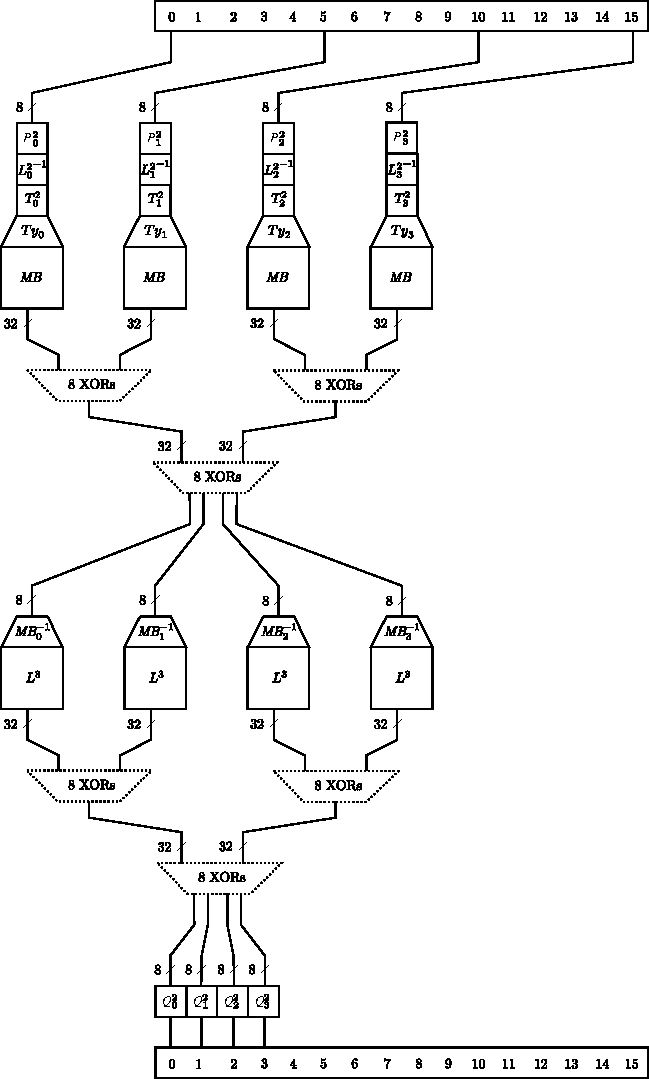
\includegraphics{WBAES_PQ.pdf}}}
	\end{center}
	\caption{Whitebox AES implementation - round \#2}
	\label{fig:wbaes}
	\end{figure*}

	Whitebox AES is AES implementation based on table lookups, functions used in AES are stored as lookup tables. Figure \ref{fig:wbaes} shows one round of whitebox AES
	implementation using lookup tables, protected with whitebox techniques like Mixing Bijections and internal encodings.

	On the diagram in figure \ref{fig:wbaes} are following whitebox functions:
	\begin{itemize}
	\item MB stands for Mixing Bijection. It is $32 \times 32$ matrix over $\text{GF}(2)$ representing linear transformation over $\text{GF}(2)$. 
	$\text{MB}^{-1}_{\{0,1,2,3\}}$ are then column stripes of corresponding MB inverse matrix - linearity is used here to perform multiplication with MB inverse matrix.
	This transformation is not interesting since it cancels out within one round. We are interested in round function R, this transformation has no effect on it.
	\item L stands also for Mixing Bijection but in this case it is $8 \times 8$ matrix over $\text{GF}(2)$ representing linear transformation over $\text{GF}(2)$. 
	Original purpose of it was to protect output of round $r$ connected to the input of round $r+1$ in table representation. 
	\item Q,P. These are random non-linear bijections in $\text{GF}(2^8)$, called internal encodings. It holds that $P^{r+1}_{i,j} \circ Q^{r}_{i,j} = id$
	\end{itemize}

	Since transformation $L$, $L^{-1}$ is performed byte-wise on state array, we can compose them with corresponding internal encodings bijections
	\begin{align}
	    Q^{r \; \prime}_{i,j} &= Q^{r}_{i,j} \circ L^{r+1}_{j} \label{eq:ioencoding_abstract_q}\\
	    P^{r \; \prime}_{i,j} &= (L^{r}_{j})^{-1} \circ P^{r}_{i,j} \label{eq:ioencoding_abstract_p}
	\end{align}

	We again obtain non-linear random bijections with embedded L transformation in it, without loss of generality. This abstraction is done in Billet's attack.


	\subsection{Whitebox Dual AES}
	There was published a paper describing AES whitebox implementation with use of dual AES. It claimed that this implementation should be harder (in terms of time complexity)
	to break using Billet's attack on whitebox AES. On the figure \ref{fig:wbaesdual} is scheme for one round, one column of state array, whitebox dual AES implementation for round 2.
	According to the original paper, in each
	column is used different generic AES. This implementation is compatible with default AES, so after computing in dual AES we have to transform the result to default AES
	with base change transformation $\Delta$.\\	
    
	% scheme for one round of WB Dual AES
	\begin{figure*}
	\begin{center}
	\leavevmode
	\centerline{\scalebox{0.9}{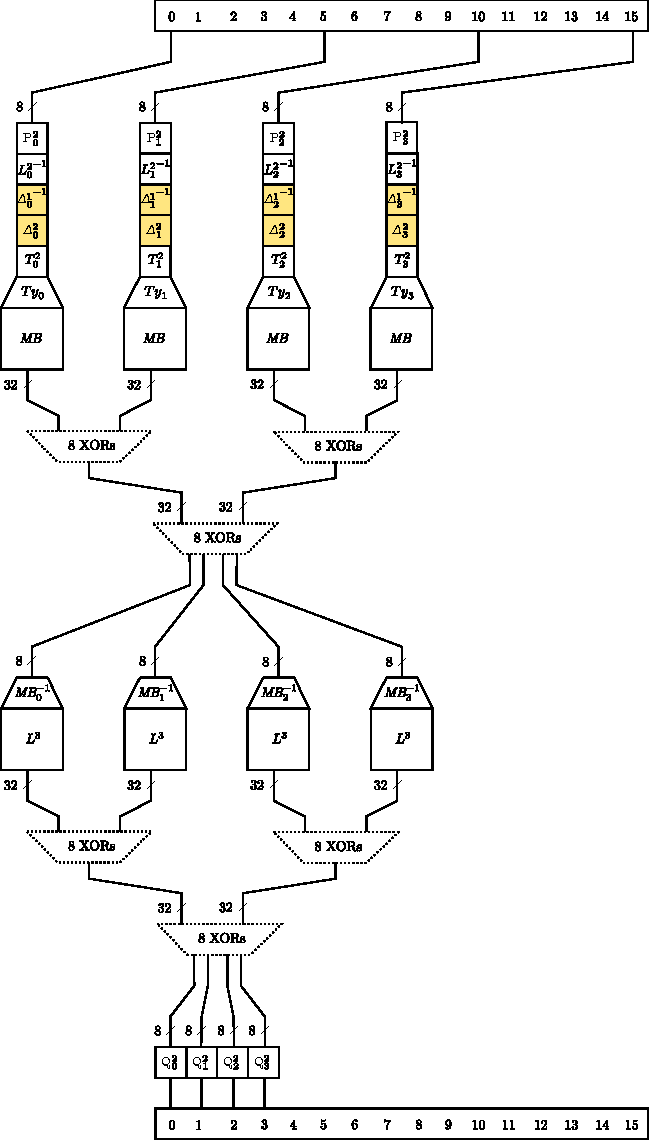
\includegraphics{WBAES_PQ_DUAL.pdf}}}
	\end{center}
	\caption{Whitebox Dual AES implementation - round \#2}
	\label{fig:wbaesdual}
	\end{figure*}



    \section{Implementation of the cipher}
    Cipher implementation description, generalization of oorschot design. Mixing bijections.

    \section{Results}
    Practical results for implementation, performance statistics, results.
    
    \section{Attack}
    My attack, see proof.tex

    \section{Attacking Dual AES scheme}
	According to \citep{Karroumi:2010:PWA:2041036.2041060} whitebox scheme using Dual AES is considered to be more difficult to crack with BGE attack and thus it is consider
	safer than original scheme proposed in \citep{Chow02white-boxcryptography}. But we show that it is not true. This result is new and was not published yet.
	
	\begin{myprop}
	Whitebox Dual AES scheme can be broken with the Billet's attack with the same time complexity as Whitebox AES scheme.
	\end{myprop}

	\begin{proof}
	Let's define round function for whitebox AES and for whitebox dual AES and compare it.

	\subsubsection*{Round function - whitebox AES}
	There are additional $Q' ,P' $ functions, input and output bijections, for details see \citep{Chow02white-boxcryptography} \citep{Billet:2004:CWB:2080787.2080809}.
	\begin{subequations}
	\begin{align} 
	y_{i,j}\left(x_{i,0}, x_{i,1}, x_{i,2}, x_{i,3}\right) & = Q^{r \; \prime}_{i,j}\left( \bigoplus^3_{l=0} \alpha_{l,j} \cdot S \left(P^{r \; \prime}_{i,l}\left(x_{i,l}\right) \right) \right) \\
								& = Q^{r \; \prime}_{i,j}\left( \bigoplus^3_{l=0} \alpha_{l,j} \cdot \left( A \left( \left(P^{r \; \prime}_{i,l}\left(x_{i,l}\right) \oplus k_{i,l} \right)^{-1} \right) \oplus c \right) \right) \\
								& = Q^{r \; \prime}_{i,j} \circ R_{i,j}\left(x_{i,0}, x_{i,1}, x_{i,2}, x_{i,3}\right) \label{eq:whitebox_aes_roud}
	\end{align}
	\end{subequations}

	\subsubsection*{Round function - whitebox dual AES}
	\begin{subequations}
	\begin{align} \label{eq:whitebox_dual_aes_r}
	y_{i,j}\left(x_{i,0}, x_{i,1}, x_{i,2}, x_{i,3}\right) &= Q^{r \; \prime}_{i,j}\left( \bigoplus^3_{l=0} \Delta \left(\alpha_{l,j}\right) \cdot \left( \Delta \times A \times \Delta^{-1} \left( \left(P^{r \; \prime}_{i,l}\left(x_{i,l}\right) \oplus \Delta\left(k_{i,l}\right) \right)^{-1} \right) \oplus \Delta \left(c\right) \right) \right) \\
								&= Q^{r \; \prime}_{i,j}\left( \bigoplus^3_{l=0} \Delta \left(\alpha_{l,j}        \cdot \left(               A \times \Delta^{-1} \left( \left(P^{r \; \prime}_{i,l}\left(x_{i,l}\right) \oplus \Delta\left(k_{i,l}\right) \right)^{-1} \right) \oplus c \right) \right) \right)
	\end{align}
	\end{subequations}

	Now it is easy to see whitebox dual AES correctness, moreover it is visible that the same attack breaking whitebox AES breaks whitebox dual AES scheme. From figure \ref{fig:wbaesdual}
	observe how rounds are connected to each other with respect to dual AESes. It is cearly visible in the case of the first round, where the inverse base change matrix $\Delta^{-1}$ is identity, because
	there is no previous dual AES encoding transformation in first round.

	Therefore the first round function is:
	\begin{subequations}
	\begin{align} \label{eq:whitebox_dual_aes_r_proof}
	y_{i,j}\left(x_{i,0}, x_{i,1}, x_{i,2}, x_{i,3}\right) &= Q^{r \; \prime}_{i,j}              \left( \bigoplus^3_{l=0} \Delta(\alpha_{l,j}) \cdot \left( \Delta \times A \times \Delta^{-1} \left(         \left(\Delta \circ P^{r \; \prime}_{i,l}\left(x_{i,l}\right) \oplus \Delta\left(k_{i,l}\right) \right)^{-1} \right) \oplus \Delta \left(c\right) \right) \right) \label{eq:whitebox_dual_aes_r_proof_1} \\ 
								&= Q^{r \; \prime}_{i,j}              \left( \bigoplus^3_{l=0} \Delta(\alpha_{l,j}) \cdot \left( \Delta \times A \times \Delta^{-1} \left( \Delta  \left(             P^{r \; \prime}_{i,l}\left(x_{i,l}\right) \oplus             k_{i,l}        \right)^{-1} \right) \oplus \Delta \left(c\right) \right) \right) \label{eq:whitebox_dual_aes_r_proof_2} \\
								&= Q^{r \; \prime}_{i,j}              \left( \bigoplus^3_{l=0} \Delta(\alpha_{l,j}) \cdot \left( \Delta \times A \times             \left(         \left(             P^{r \; \prime}_{i,l}\left(x_{i,l}\right) \oplus             k_{i,l}        \right)^{-1} \right) \oplus \Delta \left(c\right) \right) \right)\\
								&= Q^{r \; \prime}_{i,j} \circ \Delta \left( \bigoplus^3_{l=0}        \alpha_{l,j}  \cdot \left(               A \times             \left(         \left(             P^{r \; \prime}_{i,l}\left(x_{i,l}\right) \oplus             k_{i,l}        \right)^{-1} \right) \oplus              c        \right) \right)\\
								&= Q^{r \; \prime}_{i,j} \circ \Delta \circ R_{i,j}\left(x_{i,0}, x_{i,1}, x_{i,2}, x_{i,3}\right) \label{eq:whitebox_dual_aes_r_proof_final}
	\end{align}
	\end{subequations}

	Transformation from \ref{eq:whitebox_dual_aes_r_proof_1} to \ref{eq:whitebox_dual_aes_r_proof_2} is possible since it holds:
	\begin{align}
	    \forall x,y \in \text{GF}(2^8) \; : \; y = x^{-1} \Rightarrow \Delta \left(y\right) = \Delta \left( x^{-1} \right)
	\end{align}
	due to properties of generator and base change matrix.

	Now if we compare equations \ref{eq:whitebox_aes_roud} and \ref{eq:whitebox_dual_aes_r_proof_final}, they are very similar, 
	the only difference here is the application of base change matrix $\Delta$.

	Here we can do the similar thing we did in equations \ref{eq:ioencoding_abstract_q}, \ref{eq:ioencoding_abstract_p} where we composed
	two transformations, non-linear and linear to non-linear transformation, with equation \ref{eq:whitebox_dual_aes_r_proof_final}. 

	We can thus define:
	\begin{align}
	    Q^{r \; \prime\prime}_{i,j} &= Q^{r \; \prime}_{i,j} = Q^{r}_{i,j} \circ \Delta = Q^{r}_{i,j} \circ L^{r+1}_{j} \circ \Delta \\
	    y_{i,j}\left(x_{i,0}, x_{i,1}, x_{i,2}, x_{i,3}\right) &= Q^{r \; \prime}_{i,j}       \circ \Delta \circ R_{i,j}\left(x_{i,0}, x_{i,1}, x_{i,2}, x_{i,3}\right) \\
	    y_{i,j}\left(x_{i,0}, x_{i,1}, x_{i,2}, x_{i,3}\right) &= Q^{r \; \prime\prime}_{i,j} \circ R_{i,j}\left(x_{i,0}, x_{i,1}, x_{i,2}, x_{i,3}\right) \label{eq:whitebox_dual_aes_round}
	\end{align}

	Now it is evident that equations for whitebox AES \ref{eq:whitebox_aes_roud} and \ref{eq:whitebox_dual_aes_round} are the same, the only difference is only in non-linear 
	transformations $Q$, but it is important they are both non-linear. 

	Conslusion is if attack can break whitebox AES scheme with round function \ref{eq:whitebox_aes_roud} it can also break whitebox dual AES cheme. During the attack is transformation $Q$ 
	fully determined, we verified that if Dual AES scheme is used, transformation $Q$ is the exact form as described above.
	\end{proof}

    \section{Implementation of the attack}
    Attack implementation description

    \section{Attack results}
    Practical results for attack implementation, time to break.
    
    \chapter{Scheme improvement}
    The BGE attack strongly relies on publicly known constants and building blocks used in the AES cipher (MixColumn constants, fixed S-box). 
    This leads to an idea of turning constant part of cipher into key dependent ones, according to Kerckhoffs's principle. 

    It should increase computational complexity of the attack since attacker would have to try
    all combinations of key dependent part of the cipher. In the ideal scenario the attack will be unfeasible due to high computational complexity. \\
    
    As we know AES S-box is constant and has relatively simple algebraic form. In blackbox context, it is quite difficult to construct algebraic equations for whole AES (this was 
    one of design criterias of an AES in order to prevent possible algebraic attacks), but BGE attack aims only on one round of the cipher and from this perspective it is 
    quite easy to construct algebraic equations for 1 round - as we seen in BGE attack, what makes AES vulnerable to algebraic attacks in whitebox context.\\
    
    In whitebox implementation of cipher we have two contrary goals - to minimize table size and to prevent attack in whitebox context. Table size is what puts quite limitations
    in implementation and on security boundaries. In one extreme case we would build lookup table for whole AES for every possible input of size 
    $\left(2^{128} \cdot 16\right) > 10^{39}$ bytes. This 
    scheme is no weaker than AES in blackbox context, so perfectly secure in whitebox context, but rather unfeasible in practice.

    As we seen in BGE attack it is easy to turn random non-linear bijections (input/output encodings), protecting table contents, to affine transformations between rounds of
    cipher, so more complicated non-linear bijections are probably not the way out of this.
    
    The main idea here is to break backward compatibility with AES (or any other well known cipher)- as it does not have proper structure for whitebox implementation, what is 
    also visible from the fact there no non-broken whitebox scheme of AES exists nowadays [CITE HERE]. 
    In literature was already proposed to design a new cipher with whitebox implementation issues in mind \citep{Billet:2004:CWB:2080787.2080809}. 

    So we took inspiration from Twofish \cite{Schneier98twofish:a} cipher which has key dependent S-boxes with rather
    complicated algebraic representations. As I emphasized before, the key idea here is to make expressing one round of cipher as algebraic equations more difficult for an attacker.
    Our first scheme is to use Twofish key dependent S-boxes in AES algorithm. 

    \section{Twofish S-boxes}
    Here observe Twofish S-boxes (from \citep{Schneier98twofish:a}) and their algebraic representation.
    \begin{subequations}\label{eq:twofish_sbox}
    \begin{align}
	s_{0,k_0,k_1}\left(x\right) &= q_1\left[q_0\left[q_0\left[x\right] \oplus k_0 \right] \oplus k_1 \right]\\
	s_{1,k_2,k_3}\left(x\right) &= q_0\left[q_0\left[q_1\left[x\right] \oplus k_2 \right] \oplus k_3 \right]\\
	s_{2,k_4,k_5}\left(x\right) &= q_1\left[q_1\left[q_0\left[x\right] \oplus k_4 \right] \oplus k_5 \right]\\
	s_{3,k_6,k_7}\left(x\right) &= q_0\left[q_1\left[q_1\left[x\right] \oplus k_6 \right] \oplus k_7 \right]
    \end{align}
    \end{subequations}
    Where $q_0, q_1$ are fixed 8-bit permutations, $k_i,\; i \in [0,7]$ are key bytes, $s_{j,k_a,k_b},\; j \in [0,4]$ are resulting S-boxes.

    Thus instead of fixed AES S-box we use Twofish key dependent S-boxes. In particular we use $s_{j,k_a,k_b},\; j \in [0,4]$ instead of 4 the same constant
    S-boxes in computation of one column of state matrix - consistent approach with Twofish algorithm, in Twofish we have MDS as a diffusion element,
    here we have MixColumn operation [FIGURE HERE]. 

    In blackbox context there is disadvantage for key dependent S-boxes since it takes some time to generate them, for each encryption key, but in whitebox context
    the whole cipher is generated before use, including S-boxes, so during encryption/decryption there is no such disadvantage anymore.
   
    \section{Key schedule}
    BGE attack also make use of reversible AES key schedule to obtain encryption key. It is only needed to obtain round keys for two consecutive
    rounds of cipher in order to obtain full encryption key.

    In order to avoid this reversing we also modify key schedule.
    In particular we suggest to use hash-chains as round keys, so attacker would not be able to combine knowledge of two consecutive rounds as in BGE attack.
    
    We suggest to use \emph{bcrypt} \citep{Provos99afuture-adaptable} or \emph{scrypt} \citep{Percival_strongerkey} as a hash function for generating hash chains. The main reason is high time complexity needed to evaluate 
    such hash functions. This makes eventual bruteforcing even harder, because of low hashes per second ratio. We could
    use for example also \emph{SHA-256} hash function to generate hash chain, but nowadays there exists even special hardware for computing SHA digests 
    (ASICS chips, for Bitcoin mining), with performance 1500~G hashes per second for one device \cite{shamining_web}, bruteforcing with such device would be
    much faster. 
    
    In \cite{bcrypthash} M. Gosney used cluster made of GPUs (general purpose hardware) and benchmarked hash functions from performance perspective, for
    details see table \ref{tbl:hash_performance}. \emph{bcrypt} is by orders of magnitude slower than SHA1, almost by factor $10^6$. This makes bruteforce
    unfeasible on general purpose hardware. 

    \begin{table}
    \begin{center}
    \begin{tabular}{ l | l }
% 	\hline
	function & hashes per second \\ \hline
	SHA1     & $63$ G/s \\ \hline
	MD5      & $180$ G/s \\ \hline
	BCrypt   & $71$ K/s \\   \hline
    \end{tabular}
    \caption{Hash functions performance comparison}
    \label{tbl:hash_performance}
    \end{center} 
    \end{table}
    
    In AES-128 we have 128~bit cipher key, $k_0,\dots,k_{15}$. We define $k_i^r$ to be round key byte $i \in [0,15]$ used in round $r \in [0,10]$.
    
    We define hash function used further in our modified key schedule
    \begin{equation}
	hash\left(inp, salt\right)_{N_{bc}, N_{sha}} = bcrypt\left(N_{bc}, salt, \text{SHA-}256^{N_{sha}}\left(inp\right)\right)
    \end{equation}
    Where we have 2 security parameters in this scheme.
    $N_{bc}$ is work load for bcrypt, determines computation complexity of bcrypt hash function. $N_{sha}$ is number of nested iterations of SHA-256 function. 
    
    With this we define key schedule for our new cipher:
    \begin{equation}\label{eq:keySchedule}
    k_i^r = \left\{ 
    \begin{array}{l l} 
	hash_{N_{bc}, N_{sha}}(key, salt)_i                   & \quad \text{if $r=0$}\\
	hash_{N_{bc}, N_{sha}}(k^{r-1} \; || \;  key, salt)_i & \quad \text{otherwise}
    \end{array} \right.
    \end{equation}
    Where
    \begin{itemize}
     \item[$i$] subscript on right side stands for i-th byte of resulting hash
     \item[$key$] is encryption key, 128 bits
     \item[$k^{r-1}$] is whole round key for round $r-1$
     \item[$||$] symbol is concatenation of two binary arguments
     \item[$salt$] is arbitrary 128 bit salt used in bcrypt algorithm. This can be publicly known - published together with ciphertext or 
	in particular whitebox cipher instance.
    \end{itemize}

    Equation for $k_i^r$ is chosen with two primary goals in mind, attacker is not able to:
    \begin{enumerate}
     \item derive encryption key from two (or more) consecutive round keys. This results from infeasability of reversing hash chain. 
	We are also using computational intensive hash function so even bruteforcing is unfeasible.
     \item derive round key for $r_1-1$ or $r_2+1$ if he already have round keys for rounds $[r_1, r_2]$. Unavailability of deriving 
	round key for $r_1-1$ results from the previous argument, but here is also important that from already derived round keys we are not able to derive 	
	next ones (compared AES schedule case) since it also depends on encryption key directly.
    \end{enumerate}
    
    \section{Key bytes for S boxes}
    In order to increase strength of proposed scheme we don't use round key bytes for S-box computation directly. If someone succeds in determining 
    this round key bytes by computing proposition 3 from BGE attack for all key bytes possibilities it could help to derive the round keys.
    
    From this reason we use completely different keys for key-dependent S-boxes that in rest of the cipher.

    \begin{equation}\label{eq:keyForSbox}
    k_i^{r \; \prime} = \left\{ 
    \begin{array}{l l} 
	hash_{N_{bc}, N_{sha}}(key\; || \; "\text{magicConstant}", salt)_i                              & \quad \text{if $r=0$}\\
	hash_{N_{bc}, N_{sha}}(k^{r-1 \; \prime} \; || \; key \; || \; "\text{magicConstant}", salt)_i            & \quad \text{otherwise}
    \end{array} \right.
    \end{equation}
    
    The equation \ref{eq:keyForSbox} is the same as \ref{eq:keySchedule} with only difference of concatenation of "magicConstant". This makes 
    two hash chains (1 for round keys, 1 for S-boxes) completely different and non-transformable one to another.
   
    \section{Diffusion layer modification}\label{sec:cipher_invert_improvement}
    In section \ref{sec:cipher_invertibility} was mentioned cipher invertibility. I suggest to extend input/output space of the round function
    from 32-bits to 128-bits, raising complexity of mentioned inverting attack to $10\cdot4\cdot2^{128}$ operations. In AES one byte of state array depends
    only on 4 bytes = one column of state array. Round function of AES acts independently on 4 columns, making it easy to invert it. 

    Proposed improvement is in changing MDS (Maximum Distance Separable) matrix from $4 \times 4$ to $16 \times 16$. 
    Then would one byte of state array depend on 16 bytes, making round function 128-bit wide.

    MDS matrix acts as diffusion element in the cipher, since our cipher is of type substitution-permutation cipher, our MDS matrix 
    is represents invertible linear mapping. The important metric for its security is \emph{branch number} \citep{daemenBranch}, it gives measure on
    worst case diffusion. If the diffusion matrix has a maximal possible branch number, it is \emph{optimal}. 
    AES \citep{2002-daemen}, Twofish \citep{Schneier98twofish:a} and SHARK \citep{shark96} ciphers are using MDS matrices optimizing branch number as 
    main security measure of diffusion layer.
    
    For generating such MDS matrices is particularly interesting following proposition from SHARK cipher paper \citep{shark96} (for proof see
    original paper).
    
    \begin{myprop}
	Let C be a $(2n,\; n,\; n+1)$-code over the Galois field $\text{GF}(2^m)$. Let $G_e$  be the generator matrix of C in echelon form:
	\begin{equation}
	   Ge = \begin{bmatrix} I_{n \times n} & B_{n \times n}\end{bmatrix}
	\end{equation}
	Then C defines an optimal invertible linear mapping $\gamma$:
	\begin{equation}
	   \gamma \; : \; \text{GF}(2^m)^n \rightarrow \text{GF}(2^m)^n = X \mapsto Y = B \cdot X
	\end{equation}
    \end{myprop}
    
    Recall that $(2n,\; n,\; n+1)$-code is MDS \footnote{$(n,\;k,\;d)$-code is MDS iff $d=n-k+1$}. Reed-Solomon codes are subset of MDS codes, so their 
    parity check matrix can be used as MDS matrix, in the cipher acting as a strong diffucion element. MDS matrices derived from Reed-Solomon codes are used by many 
    ciphers, for example Twofish, Shark. 

    In our case we would be interested in $(32,\;16,\;17)$-code, to obtain $16 \times 16$ MDS matrix with wanted properties.
    
    Another way how to generate MDS matrices with is described in \citep{Roth:1985:GMM:7030.7044} using Cauchy matrices. 

    It is important to mention that ciphers using MDS matrix as diffusion element usually puts additional requirements on the MDS matrix, also optimizing
    performance and simplicity in hardware implementation. In blackbox context it is usually security/performance trade off. In whitebox context we need
    to have diffusion element very strong, so we can neglect performance point of view to increase security.
    
    Also article \cite{mds_aes} mentions AES diffusion layer modification from $4 \times 4$ to $16 \times 16$ MDS matrix, argumenting with 
    stronger security within one round, what is particularly interesting in whitebox context. They are constructing MDS matrix using Cauchy matrices. Cauchy matrices
    depends on the first row only, this increases possible diversity of $16 \times 16$ MDS matrices helping the following idea - key dependent diffusion.

    \begin{figure*}
    \begin{center}
    \leavevmode
    \centerline{\scalebox{1.2}{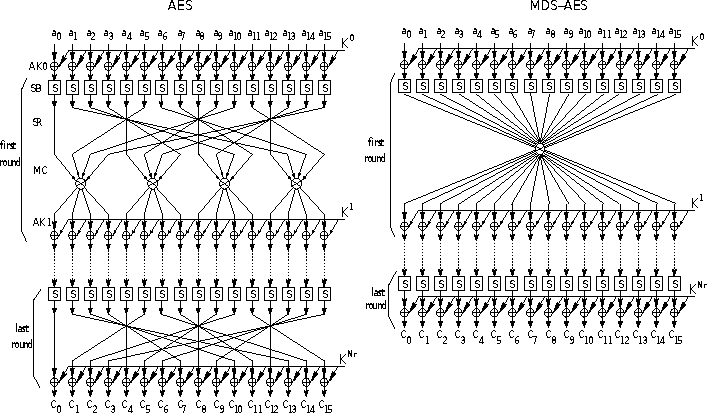
\includegraphics{AES_MDS.pdf}}}
    %\centerline{{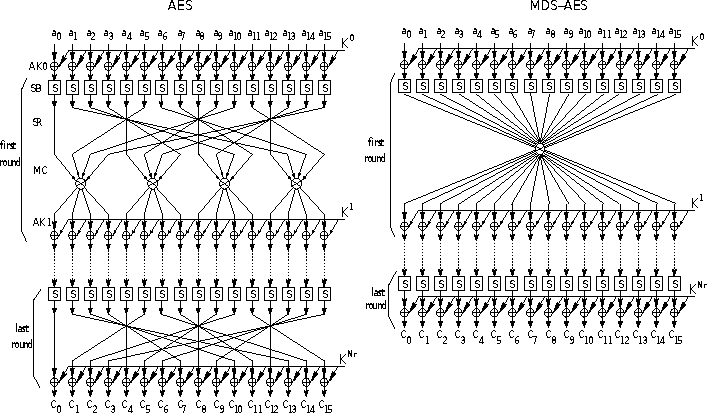
\includegraphics{AES_MDS.pdf}}
    \end{center}
    \caption{\text{Computational diagrams of AES and MDS-AES (taken from \cite{mds_aes})}}
    \label{fig:aes_mds}
    \end{figure*}
    
    Consider also idea to have key-dependent MDS matrices. If we can generate set $S_{MDS}$ of MDS matrices representing optimal linear mapping, their selection 
    can be based on key-dependent criteria. Set $S_{MDS}$ can be also extended using following proposition from \citep{journals/iacr/MalikN11}.

    \begin{myprop}
	Let $B = \left[b_{i,j} \right]_{n \times n},\; b_{i,j} \in \mathbb{F}_q$ an MDS matrix, for an element $e \in \mathbb{F}_q, \; e \neq 0$, $e \cdot B$ is an MDS matrix.
    \end{myprop}
    
    Having key-dependent diffusion layer also complicates whitebox attacks, namely Billet's \citep{Billet:2004:CWB:2080787.2080809} and 
    Generic attack by Michiels \citep{Michiels:2007:MST:1314276.1314291} requires known MDS matrix coefficients (thus key-independent).    
    
    \section{Analysis}
    In this chapter we try to analyze suggested scheme improvement from whitebox point of view, particularly we try to mount BGE attack to this modified variant. 

    S-box definitions are needed in proposition 3 in BGE attack where we obtain 4 affine mappings.
    \begin{subequations}\label{eq:BGE_prop3}
    \begin{align}
	\widetilde{P}_0 \;&: \; x \mapsto \left( S^{-1} \circ \Lambda_{\delta_0} \circ \widetilde{A}_0^{-1}\right) \left( y_0\left(x, 00, 00, 00\right) \right)\\
	\widetilde{P}_1 \;&: \; x \mapsto \left( S^{-1} \circ \Lambda_{\delta_1} \circ \widetilde{A}_0^{-1}\right) \left( y_0\left(00, x, 00, 00\right) \right)\\
	\widetilde{P}_2 \;&: \; x \mapsto \left( S^{-1} \circ \Lambda_{\delta_2} \circ \widetilde{A}_0^{-1}\right) \left( y_0\left(00, 00, x, 00\right) \right)\\
	\widetilde{P}_3 \;&: \; x \mapsto \left( S^{-1} \circ \Lambda_{\delta_3} \circ \widetilde{A}_0^{-1}\right) \left( y_0\left(00, 00, 00, x\right) \right)
    \end{align}
    \end{subequations}
    
    In our implementation of the BGE attack we iterate over $\left(\delta_i, c_i\right)_{i=0,\dots,3} \in \text{GF}(2^8)\times\text{GF}(2^8)$ what gives complexity $2^{16}$ for one mapping.
    In each step is mapping checked for affinity in $2^8$ steps (for affinity check algorithm see \ref{appendix:affcheck}), altogether one relation takes $2^{24}$ steps, for all relations
    $2^{26}$ steps.
    
    Here is the place where we use public knowledge of AES S-Box definitions. One way how to mount BGE attack to this modiffied variant is to guess also particular S-box
    mapping for each $\widetilde{P}$ and to test for its affinity. 
    
    Equations \ref{eq:twofish_sbox} describe Twofish S-boxes. There are $2^{16}$ possible $s_0$ S-boxes. One S-box mappings stored as lookup table takes $2^8$ bytes.
    Thus pre-computed $s_0$ s-box for all possible key bytes would take $2^8 \cdot 2^{16} = 2^{24} > 10^7$ bytes. 
    
    Even if attacker determines round keys for S-boxes it will be completely useless for further extraction of cipher key since hash chains are different. 
    
    Twofish S-boxes thus increase complexity of proposition 3 from BGE from $2^{24}$ to $2^{40}$. This is still not strong enough, it is highly parallelizable problem.
    In order to increase work needed to mount proposition 3 attack one could redefine key-dependent S-boxes to increase attack complexity to level $2^{128}$ what is larger
    than best known attack on AES. We then would S-box need to depend on 13 bytes derived from encryption key. Upper bound on number of different non-linear Sboxes is $256! \approx 8,5\cdot 10^{506}$ so there are still options to expand 
    S-box space. 
    
    \begin{equation}\label{eq:complex_sbox}
	s^{\prime}_{j}\left(x\right) = sboxgen(j,12,x)
    \end{equation}
    
    Where S-box is generated recursively by $sboxgen$, following the idea of nesting fixed permutations with addition of round key:
    
    \begin{equation}\label{eq:sboxgen}
	sboxgen(j,l,x) = \left\{ 
	\begin{array}{l l}  
	    q^{\prime}_{j,0}\left[ x \right]                          \oplus k_{j+1}		            & \quad \text{if $l=0$}\\
	    q^{\prime}_{j,l}\left[sboxgen\left(j, l-1,x\right)\right] \oplus k_{(j+1) \cdot (l+1)}          & \quad \text{otherwise}
	\end{array} \right.
    \end{equation}
    
    Where $q^{\prime}_{j,l}$ is one of two fixed Twofish 8-bit permutations. Particular sequence of nested permutations would require deeper analysis, to avoid possible weaknesess 
    induced by composing inapropriate permutations together, but we can choose for example:
    \setcounter{MaxMatrixCols}{13}
    \begin{subequations}
    \begin{align}
	q^{\prime}_{0} &= \begin{bmatrix}  q_1 & q_0 & q_1 & q_0 & q_1 & q_0 & q_1 & q_0 & q_1 & q_0 & q_1 & q_0 & q_0 \end{bmatrix}\\
	q^{\prime}_{1} &= \begin{bmatrix}  q_1 & q_1 & q_0 & q_0 & q_1 & q_1 & q_0 & q_0 & q_1 & q_1 & q_0 & q_0 & q_1 \end{bmatrix}\\
	q^{\prime}_{2} &= \begin{bmatrix}  q_0 & q_0 & q_1 & q_1 & q_0 & q_0 & q_1 & q_1 & q_0 & q_0 & q_1 & q_1 & q_0 \end{bmatrix}\\
	q^{\prime}_{3} &= \begin{bmatrix}  q_0 & q_0 & q_0 & q_1 & q_1 & q_1 & q_0 & q_0 & q_0 & q_1 & q_1 & q_1 & q_1 \end{bmatrix}
    \end{align}
    \end{subequations}

    This gives us good security margin for BGE attack, raising computational complexity to $2^{128}$. 
    Pre-computed $s_0$ S-box for all possible key bytes would take $2^8 \cdot 2^{8\cdot13} = 2^{112} > 10^{33}$ bytes. 

    Also as long as are SHA-256 and bcrypt uncracked, key extraction should be unfeasible, since it is not possible
    to invert hash function easily. 

    Cipher modification that affects only S-boxes and round keys, so other parts of the BGE attack are not affected, namely transforming non-linear parts
    to affine, propositions 1 and 2 work as before. 

    Cipher modification don't increase table sizes, because modifications made are only in S-box definitions and key schedule - both 
    parts of the cipher are already evaluated and stored in the lookup tables. Our modifications also don't affect encryption/decryption performance since the only
    difference is made during particular whitebox instance (lookup tables) generation. Encryption/decryption algorithm itself is not affected.
    
    \section{Analysis of diffusion layer}
    Taking also section \ref{sec:cipher_invert_improvement} into account will result also in bigger lookup tables. All table types are affected, in particular type 2, previously 
    it was mapping $2^8 \rightarrow 2^{32}$, with cascade of XOR tables to sum $4 \; \times\; 32$-bit values to obtain one column of state array. Now type 2 tables are
    $2^8 \rightarrow 2^{128}$, with cascade of XORs to obtain whole state column vector. XOR tables takes 128-bit arguments, plus 3 additional 128-bit XOR tables 
    are needed (to sum $4 \; \times\; 128$-bit results from columns).
    
    From security point of view this modiffication also prevents inverting attack mentioned in section \ref{sec:cipher_invertibility}. Function is now too wide to be
    inverted by running over $GF(2^8)^{16}$. 
    
    Key-dependent MDS matrix also prevents mounting Billet's attack. In particular we don't know MixColumn matrix coefficients so we are not able to construct set $\beta$
    from section 3.3 in \cite{Billet:2004:CWB:2080787.2080809}. This leads to further ambiguities so proposition 2 and 3 won't work anymore. This also makes recovering 
    affine parts of I/O encodings unfeasible, using this attack. But proposition 1 still works, random I/O bijections can be converted fo affine ones quite easilly.

    As noted above, also  Generic attack by Michiels \citep{Michiels:2007:MST:1314276.1314291} requires known MDS matrix coefficients.
    
    \section*{Drawbacks}
    By modification of AES design we are comming up with new cipher, what brings also some possible problems. AES and Twofish have advantage of being well analyzed from blackbox 
    context and being relatively secure. Designing a new cipher may help with increasing security in whitebox context but there also may be weaknesess in blackbox context. 
    It would be needed to analyze the new cipher from this point of view, for example for resistance to linear or differential cryptanalysis. There is no guarantee that 
    proposed cipher modifications are strong enough to resist clasical blackbox context cryptanalysis.
    
    But when designing scheme improvements we tried to follow standard principles in designing secure block cipher, inspired by AES, Twofish, Shark and others.
    
    \section{Discussion}
    Few words about field, discussion about WB cryptography.
    
\chapter{Future work}\label{sec:futurework}
    As a future work I would like to study blackbox properties of suggested improved cipher. In particular it is worth to study S-box construction, to test
    it for possible weaknesses. It will be needed to model S-boxes as algebraic equations and to test it for fixed points, for example. One can also study this S-boxes
    and their differential / linear probability coefficients (measuring resistance of an S-box to differential / linear cryptanalysis). One can test S-boxes 
    for Square and linear approximation attacks. 
    
    Resistance to Billet's attack results from dependence on 13 round key bytes. If one shows that S-box space is smaller than assumed, it can be vulnerability 
    that can be exploited by whitebox attack. 

    I would like to examine attacks on whitebox implementations, when each round of the cipher is considered as a single mini-cipher with its own key. Whitebox
    cipher implementation then would be network of serially connected mini-ciphers. From this point of view I would be interested in resistance of the mini-ciphers
    to linear and differential cryptanalysis. 
    
    
\appendix

\chapter{Appendix A}
    \subsection{Affinity check}\label{appendix:affcheck}
    In this section we describe affininity check needed in proposition 3 of BGE attack. We are given relation $\widetilde{P}$ as a lookup table
    and the task is to test it for affinity. If $\widetilde{P}$ is affine it must hold:
    \begin{equation}
	\widetilde{P}\left(x\right) = M \times x \oplus c
    \end{equation}
    For some square matrix $M$ with coefficients from $\text{GF}(2)$ and constant $c \in \text{GF}(2^8)$ (or equivalently $8\times1$ vector with coeficients from $\text{GF}(2)$).\\
    
    By evaluating $\widetilde{P}\left(0\right) = c$ we obtain affine constant $c$ so we derive new mapping $\widetilde{P^\prime}$,
    reducing the problem to test $\widetilde{P^\prime}$ for being linear.
    \begin{equation}
	\widetilde{P^\prime} \left(x\right) = \widetilde{P}\left(x\right) \oplus c
    \end{equation}
   
    And from linearity the following formula must hold:
    \begin{equation}
	\forall x \in \text{GF}(2^8), \; \exists! \; k_j \in \{0,1\}, \; j \in [0,7] \; : \; x = \sum_{j=0}^{7} k_j \cdot \widetilde{P^\prime} \left(e_j\right) \; 
    \end{equation}
    It says that each element from the field has to be unique sum of its basis vectors. Assuming that $\widetilde{P^\prime}$ is linear,
    we can obtain mapped base vectors for this transformation easily as $g_j = \widetilde{P^\prime}\left(e_j\right)$. Now it is visible that time complexity is $2^8$.
    
    \begin{algorithm}
       \caption{Algorithm for testing given mapping for being affine}
	\begin{algorithmic}[1]
	    \Function{isAffine}{$\widetilde{P} : \text{GF}(2^8) \mapsto \text{GF}(2^8)$}\Comment{Determine if P is affine mapping}
	    \State $c \gets \widetilde{P}[0]$\Comment{$c$ is affine constant}
	    \State $\widetilde{P^{\prime}}[x] \gets \widetilde{P}[x] + c$\Comment{$2^8$ time complexity}
	    \State $isAffine \gets true$
	    \For{$x\gets 0, (2^8-1)$}
		\State $px\gets \widetilde{P^{\prime}}[x]$
		\State $cx\gets 0$
		\For{$i\gets 0, 7$}
		    \If{$x_{i} = 1$}\Comment{$x_{i}$ is $i$-th bit of x in binary}
			\State $cx \gets cx \oplus \widetilde{P^{\prime}}\left[e_i\right]$\Comment{$ \widetilde{P^{\prime}}\left[e_i\right]$ is mapped base vector}
		    \EndIf
		\EndFor
		\If{$ px\neq cx $}\Comment{$cx$ is expressed via mapped base vectors}
		    \State $isAffine \gets false$
		    \State \textbf{return}
		\EndIf
	    \EndFor\Comment{All elements from field checked for linearity}
	    \State \textbf{return} $isAffine$
	    \EndFunction
	\end{algorithmic}
	\label{alg:affineTest}
    \end{algorithm}

    % bibtex here
    \addcontentsline{toc}{chapter}{Bibliography}
    \pagestyle{plain}
    \bibliography{thesis}
    

%\begin{thebibliography}{9}
%	\bibitem{twofish} \uppercase{SCHNEIRER, B. KELSEY, J., Whiting, D., Wagner, D., Hall, C., Ferguson, N.} , Twofish: A 128-Bit Block Cipher \textless\url{http://www.schneier.com/paper-twofish-paper.pdf}, cited~14.05.2012.
%	\bibitem{bcrypt} \uppercase{Provos, N., Talan Jason Sutton, T. J.} {\it A Future-Adaptable Password Scheme.} Proceedings of 1999 USENIX Annual Technical Conference: 81--92.
%	\bibitem{shamining} Butterfly labs \textless\url{https://products.butterflylabs.com} cited~14.05.2012.
%	\bibitem{bcrypthash} \uppercase{Gosney, J. M.} Password Cracking HPC , Passwords\^12 Security Conference, 2012. Available at \textless\url{http://passwords12.at.ifi.uio.no/Jeremi_Gosney_Password_Cracking_HPC_Passwords12.pdf}
%	\bibitem{wsn} AGHAVENDRA, C., SIVALINGAN, KRISHNA M. {\it Wireless Sensor Networks}. Springer, 2004. ISBN~978-0-387-35269-5.
%	\bibitem{abat} HARTER, A., et al. {\it The anatomy of a~context-aware application.} Proceedings of the 5th Annual ACM/IEEE International Conference on Mobile Computing and Networking (Mobicom '99), Seattle, Washington, USA, August 15-20 1999. New York, NY, USA: ACM, 1999. str.~59--68. ISBN~1-58113-142-9. doi:~10.1145/313451.313476.
%	\bibitem{cricket} PRIYANTHHA, N., CHAKRABORTY, A., BALAKRISHNAN, H. {\it The Cricket Location-Support System.} Proceedings of the 6th annual international conference on Mobile computing and networking (ACM MOBICOM), Boston, MA, August 2000. New York, NY, USA: ACM, 1999. str.~32--43. ISBN~1-58113-197-6. doi:~10.1145/345910.345917.
%	\bibitem{trilateration} KAMINSKY A. {\it Trilateration.} \textless\url{http://www.cs.rit.edu/~ark/543/module05/trilateration.pdf}\textgreater 2007, cit.~5.5.2011.
% 	\bibitem{trans_standard} IEEE {\it IEEE std. 802.15.4 - 2006: Wireless Medium Access Control (MAC) and Physical Layer (PHY) specifications for Low Rate Wireless Personal Area Networks (LR-WPANs).} \textless\url{http://standards.ieee.org/getieee802/download/802.15.4-2006.pdf}\textgreater 2006, cit.~5.5.2011.	
% 	\bibitem{antenna} \uppercase{Christodoulou, C.G. and Wahid, P.F.} {\it Fundamentals of antennas: concepts and applications}. SPIE Press, 2001. str.~13. ISBN~9780819441126.
% 	\bibitem{reactive} \uppercase{Seybold, J.S.} {\it Introduction to RF propagation}. Wiley, 2005. ISBN~9780471655961.
% 	\bibitem{fraunhofer_small_antenna} \uppercase{Cincinnati Technical Center} {\it Electromagnetic radiation and how it affects your instruments}. \textless\url{http://www.osha.gov/SLTC/radiofrequencyradiation/electromagnetic\_fieldmemo/electromagnetic.html}\textgreater 2011. cit.~5.5.2011.
% 	\bibitem{rappaport1996wireless} \uppercase{Rappaport, T.S.} {\it Wireless communications: principles and practice}. Prentice Hall PTR, 1996. str.~69--196. ISBN~9780133755367.
% 	\bibitem{fresnel} \uppercase{Stavrou, S. and Saunders, S.R.} {\it Factors influencing outdoor to indoor radio wave propagation.} Antennas and Propagation, 2003. (ICAP 2003). Twelfth International Conference on (Conf. Publ. No. 491). str.~581--585 vol 2. doi:~10.1049/cp:20030142.
% 	\bibitem{wirelessAndrea} \uppercase{Goldsmith, A.} {\it Wireless communications}. Cambridge University Press, 2005. str.~ 383--392,404--414,427. ISBN~9780521837163.
% 	\bibitem{nearfar} \uppercase{Hadzi-Velkov, Z., Spasenovski B.} {\it Capture Effect in IEEE 802.11 Basic Service Area Under Influence of Rayleigh Fading and Near/Far Effect}. IEEE Internation Symposium on Personal Indoor Communication, 2002.
% 	\bibitem{nearfar_indoor} \uppercase{Whitehouse, K. and Woo, A. and Jiang, F. and Polastre, J. and Culler, D.} {\it Exploiting the capture effect for collision detection and recovery.} Proceedings of the 2nd IEEE workshop on Embedded Networked Sensors, Washington, DC, USA, 2005. IEEE Computer Society, 2005. str.~45--52. ISBN~0-7803-9246-9.
% 	\bibitem{multipath} \uppercase{Sohraby, K. and Minoli, D. and Znati, T.F.} {\it Wireless sensor networks: technology, protocols, and applications}. Wiley-Interscience, 2007. str.~90--101. ISBN~9780471743002.
% 	\bibitem{positionLocation} \uppercase{Mu{\~n}oz, D. and Vargas, C.} {\it Position location techniques and applications}. Academic Press, 2009. ISBN~9780123743534.
% 	\bibitem{apache_common} \uppercase{Appache commons} {\it Commons-Math: The Apache Commons Mathematics Library} 2011, \textless\url{http://commons.apache.org/math/}\textgreater 2001, cit.~5.5.2011.
% 	\bibitem{numerical} \uppercase{Nocedal, J. and Wright, S.J.} {\it Numerical optimization.} Springer, 1999. str.~250--274. ISBN~9780387987934.
% 	\bibitem{lm} \uppercase{Gershenfeld, N.A.} {\it The nature of mathematical modeling}. Cambridge University Press, 1999. ISBN~9780521570954.
% 	\bibitem{winklerMovingAverage} \uppercase{Winkler Z.} {\it Měření rychlosti.} Dostupné z~World Wide Web: \textless\url{http://robotika.cz/guide/filtering/en}\textgreater, cit.~5.5.2011.
% 	\bibitem{trilateration_robot} \uppercase{Zhou, Y.} {\it An efficient least-squares trilateration algorithm for mobile robot localization.} Proceedings of the 2009 IEEE/RSJ international conference on Intelligent robots and systems, IROS'09, St. Louis, MO, USA. IEEE Press, 2009. str.~3474--3479. ISBN~978-1-4244-3803-7.
% 	\bibitem{thomas_robotLocalization} \uppercase{Thomas, F. and Ros, L.} {\it Revisiting trilateration for robot localization.} IEEE Transactions on robotics vol. 21, Feb. 2005. str.~93--101. doi:~\mbox{10.1109/TRO.2004.833793}.
% 	\bibitem{overdetermined} Wikipedia, the free encyclopedia: {\it Overdetermined system}. \textless\url{http://en.wikipedia.org/wiki/Overdetermined_system}\textgreater, cit.~5.5.2011.
% 	\bibitem{farahani2008zigbee} \uppercase{Farahani, S.} {\it ZigBee wireless networks and transceivers.} Newnes/Elsevier, 2008. str.~229--231. ISBN~9780750683937.
% 	\bibitem{tmote_datasheet} \uppercase{Moteiv Corporation.} {\it Telos (rev B):PRELIMINARY Datasheet.} 2004. \textless\url{http://www.bandwavetech.com/download/tmote-sky-datasheet.pdf}\textgreater 2004, cit.~5.5.2011.
% 	\bibitem{tinyos} {\it TinyOS Documentation Wiki.} \textless\url{http://docs.tinyos.net/index.php/}\textgreater 2011, cit.~5.5.2009.    %http://www.tinyos.net/
% 	\bibitem{invertedf01} \uppercase{Andersen A.} {\it 2.4GHz Inverted F Antenna, Design note DN0007}, 2008. \textless\url{http://focus.ti.com.cn/cn/lit/an/swru120b/swru120b.pdf}\textgreater 2008, cit 5.5.2011.
% 	\bibitem{printantena} WATERHOUSE, R. B. {\it Printed antennas for wireless communications}. Wiley, 2007. ISBN~047051069.
% 	\bibitem{invertedFGain} \uppercase{Raman, B., Chebrolu, K., Madabhushi, N., Go, D. Y., Valiveti, P. K.k and Jain, D.,} {\it Implications of link range and (In)stability on sensor network architecture}, Proceedings of the 12th annual international conference on Mobile computing and networking , Los Angeles, CA, USA, pp. 65-72, 2006.
% 	\bibitem{cc2420} \uppercase{Chipcon}, {\it 2.4 GHz IEEE 802.15.4 / ZigBee-ready RF Transceiver.} str.~11,~48--49. \textless\url{http://focus.ti.com/lit/ds/symlink/cc2420.pdf}\textgreater 2009, cit.~5.5.2011. 
% 	\bibitem{tos_message} \uppercase{Levis P.} {\it message\_t} \textless\url{http://www.tinyos.net/tinyos-2.x/doc/html/tep111.html}\textgreater 2011, cit.~5.5.2011.
% 	\bibitem{sht1x_datasheet} \uppercase{Sensirion.} {\it Datasheet SHT1x (SHT10, SHT11, SHT15). Humidity and Temperature Sensor} 2010. \textless\url{http://www.sensirion.com/en/pdf/product_information/Datasheet-humidity-sensor-SHT1x.pdf}\textgreater 2010, cit.~5.5.2011.
% 	\bibitem{dePbloThesis} \uppercase{Escol\`{a} A.} {\it Development of a wireless sensor network with 6LoWPAN support.} Dostupné z~World Wide Web: \textless\url{http://upcommons.upc.edu/pfc/bitstream/2099.1/7806/1/memoria.pdf}\textgreater, cit.~5.5.2011.
% 	\bibitem{rss_localization_study} \uppercase{De Cauwer, P. Van Overtveldt, T., Doggen, J., Van der Schueren, F. Weyn, M., Bracke, J.} {\it Study of RSS-Based Localisation Methods in Wireless Sensor Networks.} Proceeding of the Fourth European Conference on the Use of Modern Information and Communication Technologies, Gent, Beglium, 2010. 
% 	\bibitem{s1} PATWARI, N., HERO, A. {\it Using proximity and quantized RSS for sensor.} Proceedings of the 2nd ACM international conference on Wireless sensor networks and applications, San Diego, CA, USA, 2003. New York, NY, USA: ACM, 2003. str.~20--29. ISBN~1-58113-764-8. doi:~10.1145/941350.941354.
%         \bibitem{s2} ELNAHRAWY, E., LI, X.,MARTIN, R. {\it The limits of localization using RSS.} Proceedings of the 2nd international conference on Embedded networked sensor systems, Baltimore, MD, USA, 2004. New York, NY, USA: ACM, 2004. str.~283--284. ISBN~1-58113-879-2. doi:~10.1145/1031495.1031537.
% % 	\bibitem{neuro} GURNEY, K., GURNEY, K. {\it An introduction to neural networks}. UCL Press, 1997. ISBN~1-85728-503-4.
% 	\bibitem{probab} FULLER, R., KOUTSOUKOS, D. {\it Mobile Entity Localization and Tracking in GPS-less Environnments.} Second International Workshop, MELT~2009, Orlando, FL, USA, September 30, 2009, Springer, 2009. str.~66--78.
% 	\bibitem{sqlitejdbc} Zentus, {\it SqliteJDBC} 2011, \textless\url{http://www.zentus.com/sqlitejdbc}\textgreater, cit.~5.5.2011.
% 	\bibitem{sqlite} SQLite \textless\url{http://www.sqlite.org}\textgreater, cit.~5.5.2011.
% 	\bibitem{jfreechart} \uppercase{Gilbert D.} {\it JFreeChart} 2011, \textless\url{http://www.jfree.org/jfreechart}\textgreater, cit.~5.5.2011.
% 	\bibitem{bsdlicense} University of California, Berkeley {\it BSD License}, \textless\url{http://www.opensource.org/licenses/bsd-license.php}\textgreater, cit.~5.5.2011.
% 	\bibitem{gnulgpl} {\it GNU Lesser General Public License}, \textless\url{http://www.gnu.org/copyleft/lesser.html}\textgreater, cit.~5.5.2011.
% 	\bibitem{apachelicence} Apache commons {\it The Apache Software License, version 2}, \textless\url{http://commons.apache.org/math/license.html}\textgreater, cit.~5.5.2011.
% 	%images
% % 	\bibitem{img_fresnel_zones} Fresnelove zóny, \textless\url{http://www.zytrax.com/tech/wireless/fresnel.htm}\textgreater, cit.~2.5.2011.
% 	\bibitem{img_skm_studyroom} Požiarny evakuačný plán 11. poschodia SKM MU, Bratří Žůrku 5, Brno.
	
%       citovanie el.
%         \bibitem{varekova} Svobodová Vařeková, R.: {\it PV082 Computational chemistry} [online].  Dostupné z~World Wide Web: \textless\url{http://ncbr.chemi.muni.cz/~svobodova/vyuka/pocitacova_chemie/}\textgreater
%         \bibitem{cjmol} {\it Jmol} [online]. Dostupné z~World Wide Web: \textless\url{http://jmol.sourceforge.net/}\textgreater
%        wiki
%         \bibitem{cjvm} Wikipedia, the free encyclopedia: {\it Java Virtual Machine}. Dostupné z~World Wide Web: \textless\url{http://en.wikipedia.org/wiki/Java_Virtual_Machine}\textgreater


	%\bibitem{cc2420} http://inst.eecs.berkeley.edu/~cs150/Documents/CC2420.pdf
	%\bibitem{nesc} nesC: {\it A Programming Language for Deeply Networked Systems.} \textless\url{http://nescc.sourceforge.net/}\textgreater.
	%\bibitem{multilat} FERRARRI, G. {\it Sensor Networks: Where Theory Meets Practice}. Springer, 2010. str.~260--264. ISBN~3-64201-340-6.
	%\bibitem{knear} ABRAHAM, A., LIANG, Y. {\it Computational intelligence in medical informatics}. Springer, 2008. str.~190--191. ISBN~3-54075-767-8.
	%\bibitem{channels} IEEE P802.15 Working Group {\it IEEE Std 802.15.4-2006: Part 15.4: Wireless Medium Access Control (MAC) and Physical Layer (PHY) Specifications for Low-Rate Wireless Personal Area Networks (WPANs).} New York, NY, USA: IEEE, 2006. str.~45--50. ISBN~0-7381-4996-9.	
%\end{thebibliography}
\end{document}

% % % % % 
% % % % %  TEXHELP
% % % % % 
% \,		(thinspace)
% \;		(thickspace)
% \quad   	(quadspace)
% \qquad  	(double quadspace)
% \!		(negative thinspace)
% 
% % % 
% % % FLOATS
% % % 
% % You can force LaTeX to ignore most of the parameters for one specific float occurrence by including an exclamation mark (!) in the placement parameters, e.g. 
% % \begin{figure}[!htb]
% % 
% % Floats which contain a ``t'' in the position parameter could be placed before the place where they are referenced (but on the same page). This is normal behaviour for LaTeX but some people just don't like it. There are a number of ways to prevent this: 
% % Of course deleting the ``t'' will help, but in general this is undesirable, as you may want the float to be placed at the top of the next page. 
% % use the flafter package which causes floats never to be placed ``backwards''. 
% % use the command \suppressfloats[t]. This command will cause floats for the top position on this page to be moved to the next page. This can also be done with [b] or without parameter for all floats on this page. 
% % 
% % If in spite of all your attempts LaTeX still moves your floats to the end of the document or the end of a chapter, you can insert a \clearpage command. This will start a new page and insert all pending floats before continueing. If it is undesirable to have a pagebreak you can use the afterpage package and the following command: 
% % \afterpage{\clearpage}
% % 
% % This will wait until the current page is finished and then flush all outstanding floats. In some pathological circumstances afterpage may give strange results, however. 
% % 
% % Finally, if you want a float only at the place where you define it, without LaTeX moving it whatsoever, you can use the float package and give the command: 
% % \restylefloat{figure}
% % in the preamble. Now you will be able to specify [H] as the position parameter, which will mean ``HERE and only HERE''. This may cause an unwanted page break however. If you want to avoid the unwanted pagebreak, i.e. let LaTeX move the float only if it doesn't fit on the page, the use the afterpage package with: 
% % \afterpage{\clearpage \begin{figure}[H] ... \end{figure}}
% % 
% % Complaints from LaTeX about ``Too many floats'' are usually caused by one of the above problems: floats not being able to be placed and LaTeX collecting too many of them. The solutions given above, especially those with \clearpage in them will usually help. In some cases there really are too many floats, as LaTeX has a limited number of ``boxes'' to store the floats. The package morefloats can be used to increase this number. If you need still more then you must edit a private copy of this file, but even then there will be some limit that you cannot pass. Then your only resort will be to change your document.